% !TeX spellcheck = en_GB
\documentclass[AERbeamer%              style
              ,optEnglish%            language
              %,handout%               deactivate animation
              ,optBiber%               bibliography tool
              ,optBibstyleAlphabetic%
              ,optBeamerClassicFormat% 4:3 format
              %,optBeamerWideFormat%   16:9 format
              ]{AERlatex}%
\setbeameroption{show notes}% Show all notes
%
% Set paths
\graphicspath{{figures_lecture_1/}}%
\addbibresource{literature.bib}%
%
% Package Imports
%\usepackage{media9}
\usepackage{graphicx}
\usepackage{multimedia}
\usepackage{subcaption}
\usepackage{amsmath}
%
% set meta data
\title{Probabilistic Programming for Scientific Discovery}%
\subtitle{Lecture 1}
\author{Ludger Paehler}% (optional)
\date{\AERutilsDate{29}{7}{2020}}% (optional)
\institute{Lviv Data Science Summer School}% (optional)
%
% Setup of header and footer
\AERbeamerSetupHeader{\AERlayoutHeaderCDChair}%
\AERbeamerSetupFooterCD%
%\AERbeamerSetupFooterSlideNumberOnly%
%
\begin{document}%
%
% Start with titlepage
\AERbeamerTitlePageDefault%
%
%\begin{frame}{Title of Slide}{Subtitle of Slide}%
%    \blindtext%
%\end{frame}%
%

% Slide 0: Table of Contents
\begin{frame}{Table of Contents}{}%
    % Contents
    \tableofcontents
\end{frame}%


% Introduction to the chair
\section{Overview of Research at the Chair}


% Christian Breitsamter
\begin{frame}[c]{Overview}{Aircraft- and Helicopter Aerodynamics, Prof.Dr. C. Breitsamter}
    \centering
    % Three columns of 3 pictures each
    \begin{columns}[T]
        % First column
        \begin{column}{0.33\textwidth}
            \begin{figure}
                \centering
                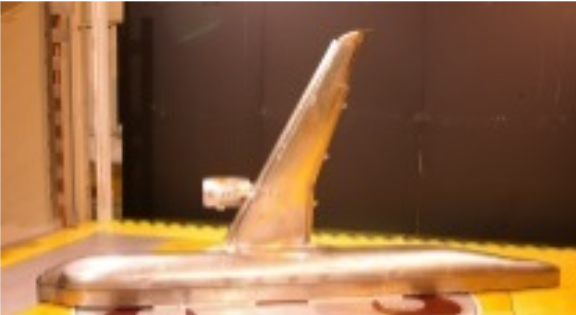
\includegraphics[width=0.8\textwidth]{Breitsamter1.png}
            \end{figure}
            \begin{figure}
                \centering
                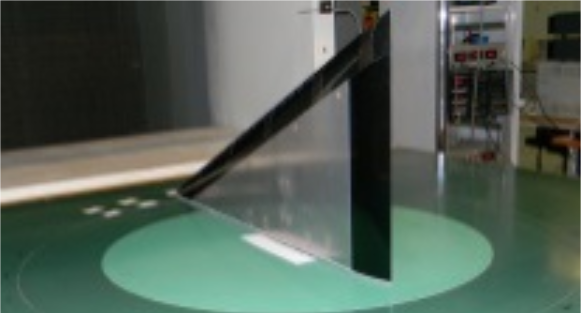
\includegraphics[width=0.8\textwidth]{Breitsamter2.png}
            \end{figure}
            \begin{figure}
                \centering
                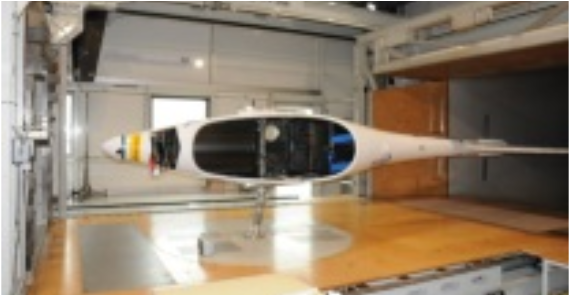
\includegraphics[width=0.8\textwidth]{Breitsamter3.png}
            \end{figure}
        \end{column}
        % Second column
        \begin{column}{0.33\textwidth}
            \begin{figure}
                \centering
                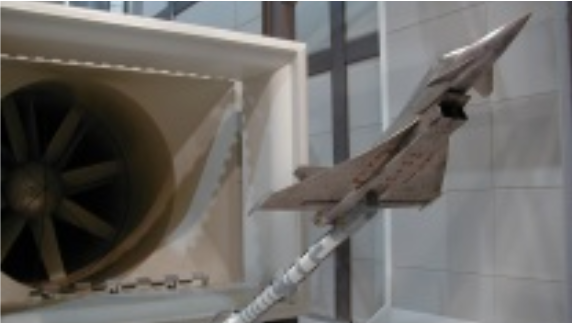
\includegraphics[width=0.77\textwidth]{Breitsamter4.png}
            \end{figure}
            \begin{figure}
                \centering
                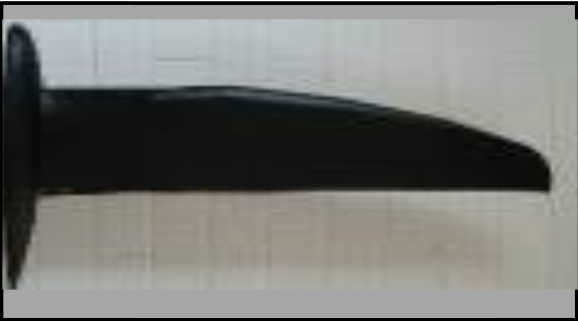
\includegraphics[width=0.77\textwidth]{Breitsamter5.png}
            \end{figure}
            \begin{figure}
                \centering
                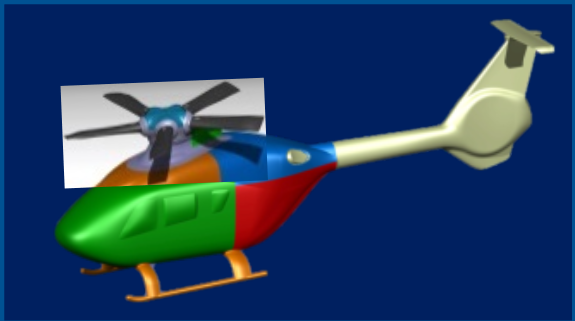
\includegraphics[width=0.77\textwidth]{Breitsamter6.png}
            \end{figure}
        \end{column}
        % Third column
        \begin{column}{0.33\textwidth}
            \begin{figure}
                \centering
                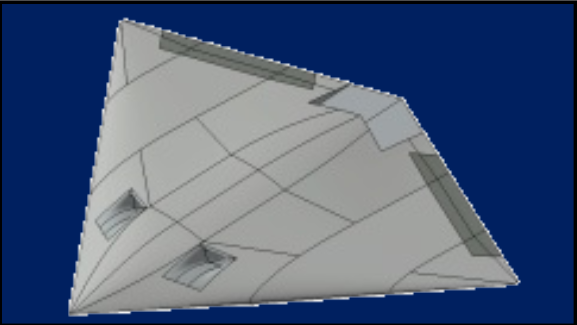
\includegraphics[width=0.77\textwidth]{Breitsamter7.png}
            \end{figure}
            \begin{figure}
                \centering
                
\includegraphics[width=0.77\textwidth]{Breitsamter8.png}
            \end{figure}
            \begin{figure}
                \centering
                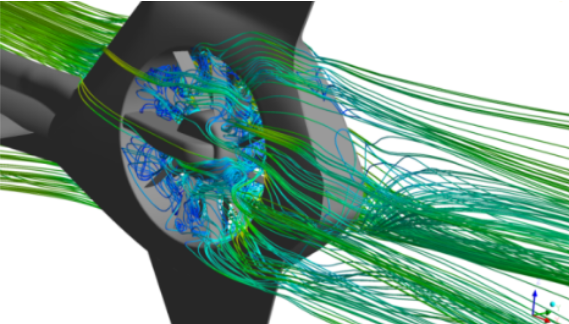
\includegraphics[width=0.77\textwidth]{Breitsamter9.png}
            \end{figure}
        \end{column}
    \end{columns}
\end{frame}


% Christian Stemmer
\begin{frame}[c]{Overview}{High-Speed Aerodynamics, apl.Prof.Dr. C. Stemmer}
    \centering
    \begin{figure}
        \centering
        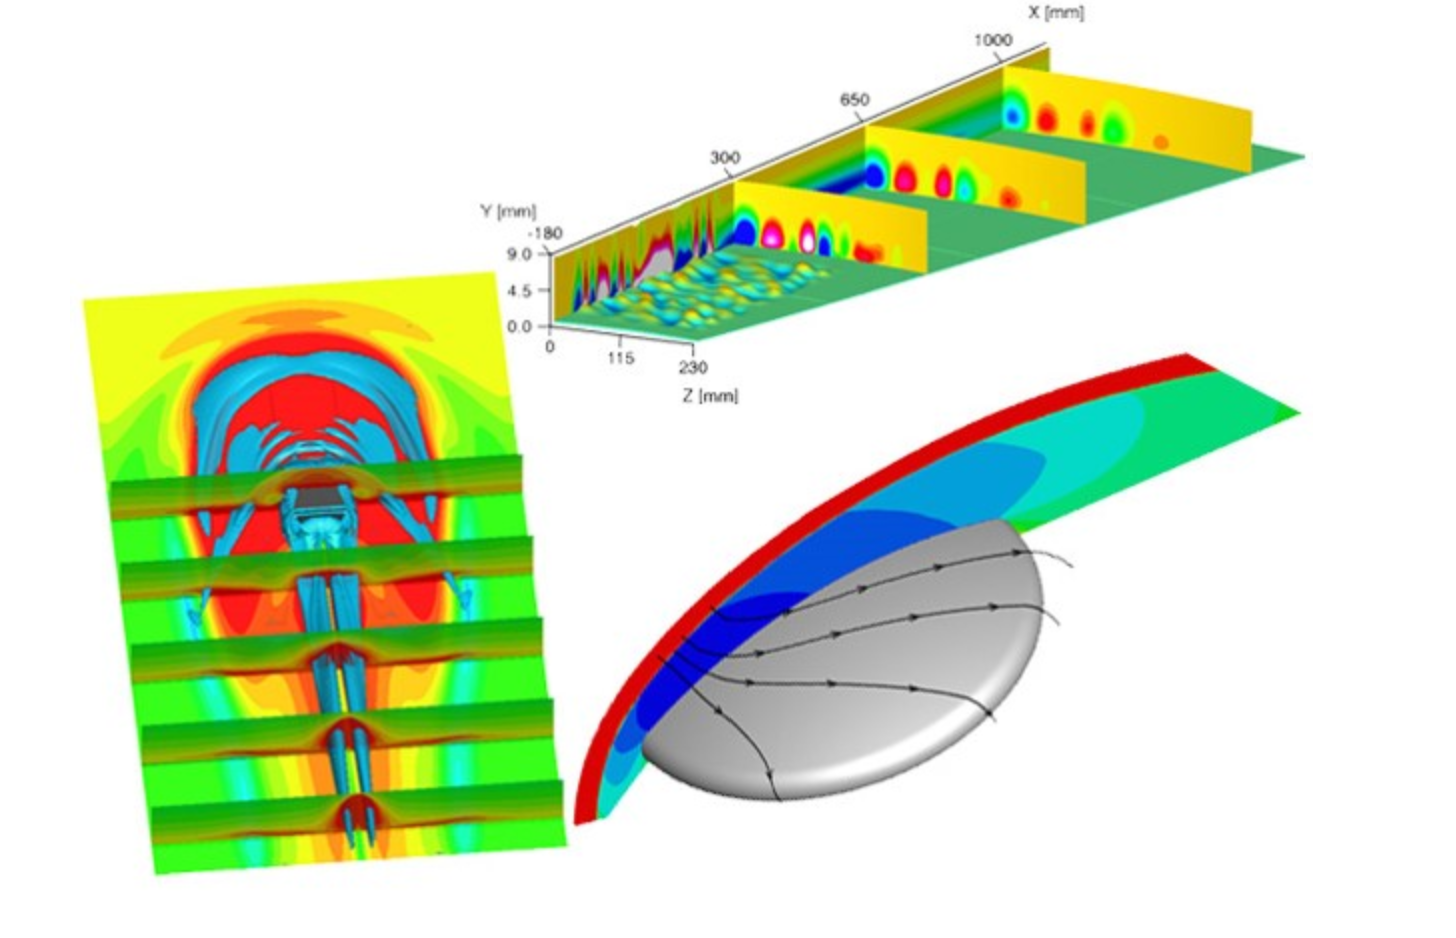
\includegraphics[width=0.7\textwidth]{Stemmer.png}
    \end{figure}
\end{frame}


% Thomas Indinger
\begin{frame}[c]{Overview}{Automotive Aerodynamics, PD Dr. T. Indinger}
    \centering
    \begin{columns}[T]
        % Text plus wind tunnel
        \begin{column}{0.48\textwidth}
            \begin{itemize}
                \item DrivAER
                \item Experimental investigation using a moving floor
                \item Numerical investigations using the lattice boltzmann method
            \end{itemize}
            \begin{figure}
                \centering
                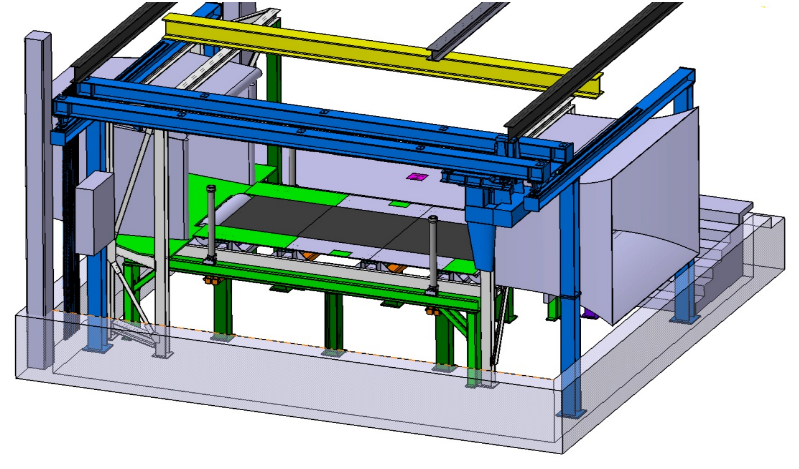
\includegraphics[width=0.8\textwidth]{Indinger1.png}
            \end{figure}
        \end{column}
        % Pictures
        \begin{column}{0.48\textwidth}
            \begin{figure}
                \centering
                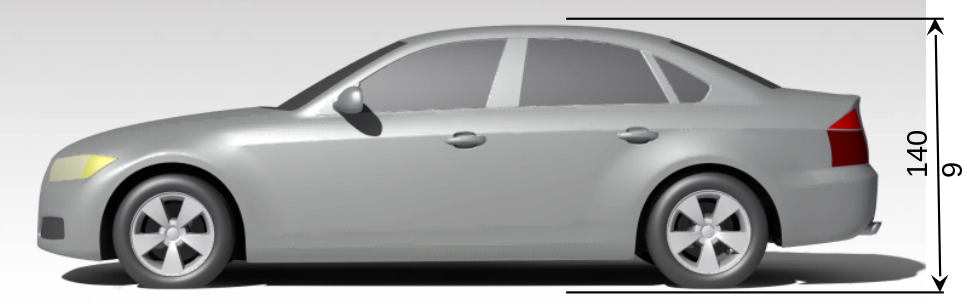
\includegraphics[width=0.8\textwidth]{Indinger3.png}
            \end{figure}
            \begin{figure}
                \centering
                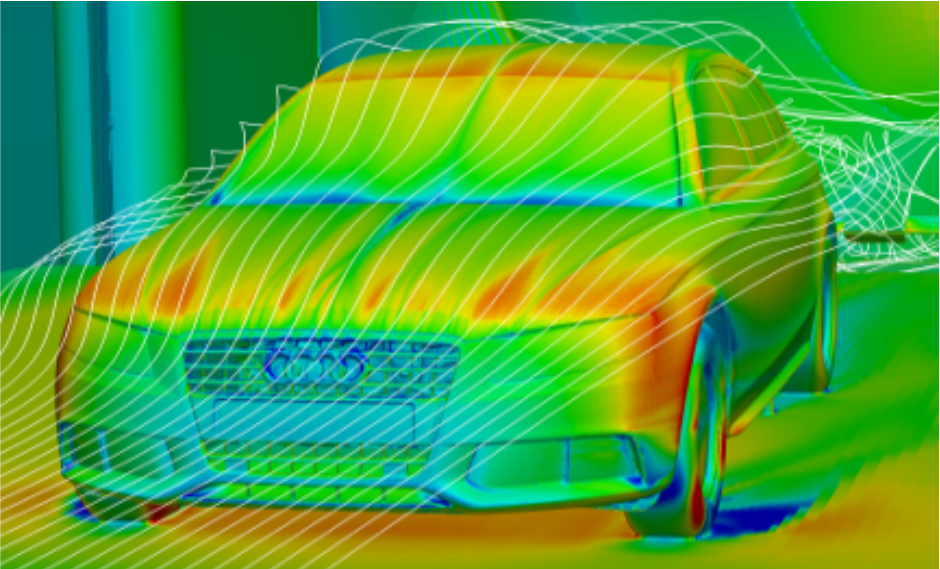
\includegraphics[width=0.8\textwidth]{Indinger2.png}
            \end{figure}
        \end{column}
    \end{columns}
\end{frame}


% Steffen Schmidt
\begin{frame}[c]{Overview}{Compressible Flows, Dr. S. Schmidt}
    \centering
    \begin{columns}[T]
        % Text plus picture
        \begin{column}{0.48\textwidth}
            \begin{itemize}
                \item Investigation of cavitation phenomena in multiphase-flows
                \item Interaction of turbulence and cavities
                \item Effects of primary jet breakup
            \end{itemize}
            \begin{figure}
                \centering
                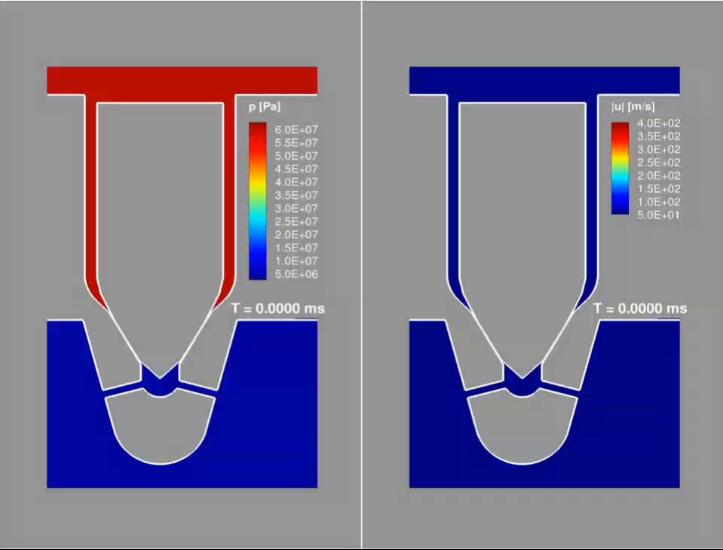
\includegraphics[width=0.8\textwidth]{Steffen1.png}
            \end{figure}
        \end{column}
        % Pictures
        \begin{column}{0.48\textwidth}
            \centering
            \begin{figure}
                \centering
                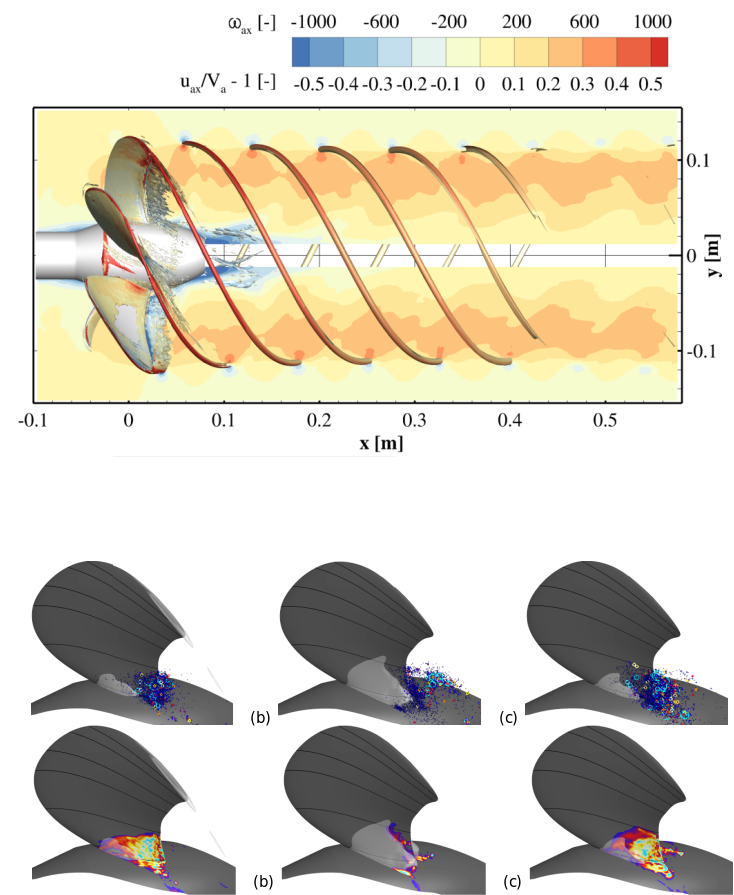
\includegraphics[width=0.8\textwidth]{Steffen2.png}
            \end{figure}
        \end{column}
    \end{columns}
\end{frame}


% Hu & Stefan Adami
\begin{frame}[c]{Overview}{Complex Fluids, PD Dr. XY Hu, Dr. S. Adami}
    \centering
    \begin{columns}[T]
        % Text plus picture
        \begin{column}{0.48\textwidth}
            \begin{itemize}
                \item Smoother particle hydrodynamics models for incompressible turbulent flows
                \item Numerical simulations of multiphase-flows using particle methods
                \item Microfluidics, Polymer and DNA solutions
                \item Waterjet- and Spray-dynamics
            \end{itemize}
            \vspace{0.75cm}
            \begin{figure}
                \centering
                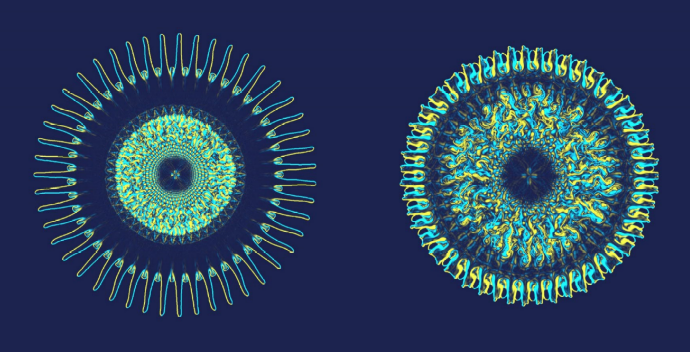
\includegraphics[width=0.8\textwidth]{ComplexFluids1.png}
            \end{figure}
        \end{column}
        % Picture
        \begin{column}{0.48\textwidth}
            \begin{figure}
                \centering
                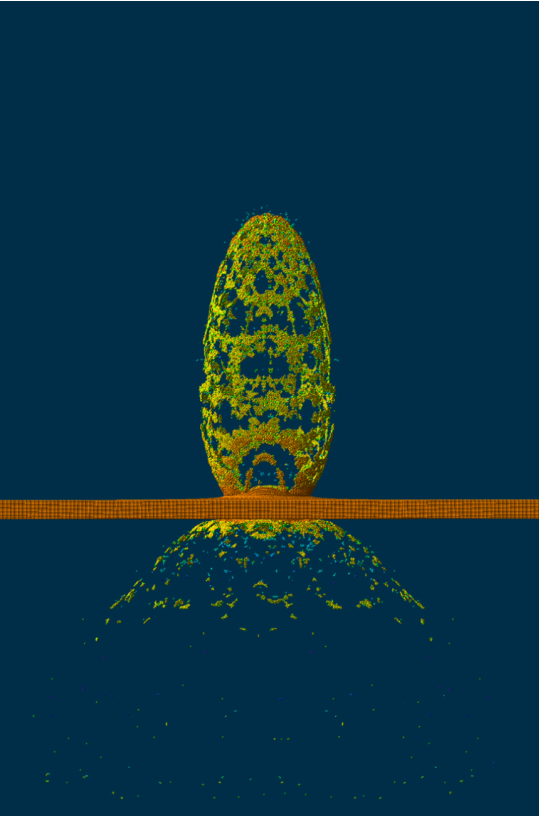
\includegraphics[width=0.6\textwidth]{ComplexFluids2.png}
            \end{figure}
        \end{column}
    \end{columns}
\end{frame}


% Nanoshock
\begin{frame}[c]{Overview}{NANOSHOCK - ERC Advanced Grant, Dr. S. Adami, Dr. M. Giglmaier}
    \centering
    \begin{columns}[T]
        % Text plus picture
        \begin{column}{0.48\textwidth}
            \centering
            \begin{itemize}
                \item Shock-induced processes in multiphase-flows
                \item Exploration of contactless flow-manipulation in processing, nanotech and medtech
            \end{itemize}
            \begin{figure}
                \centering
                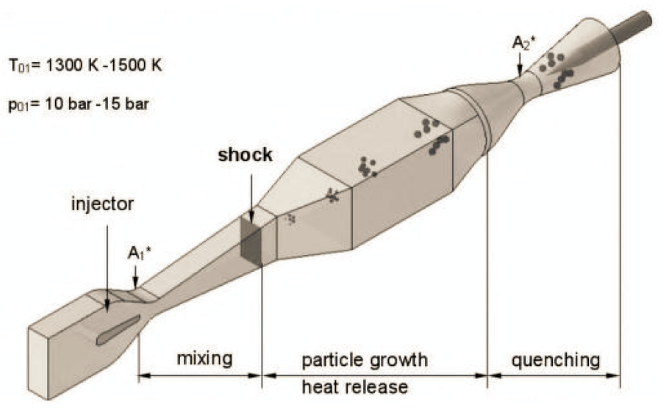
\includegraphics[width=0.8\textwidth]{Nanoshock1.png}
            \end{figure}
        \end{column}
        % Pictures
        \begin{column}{0.48\textwidth}
            \centering
            \begin{figure}
                \centering
                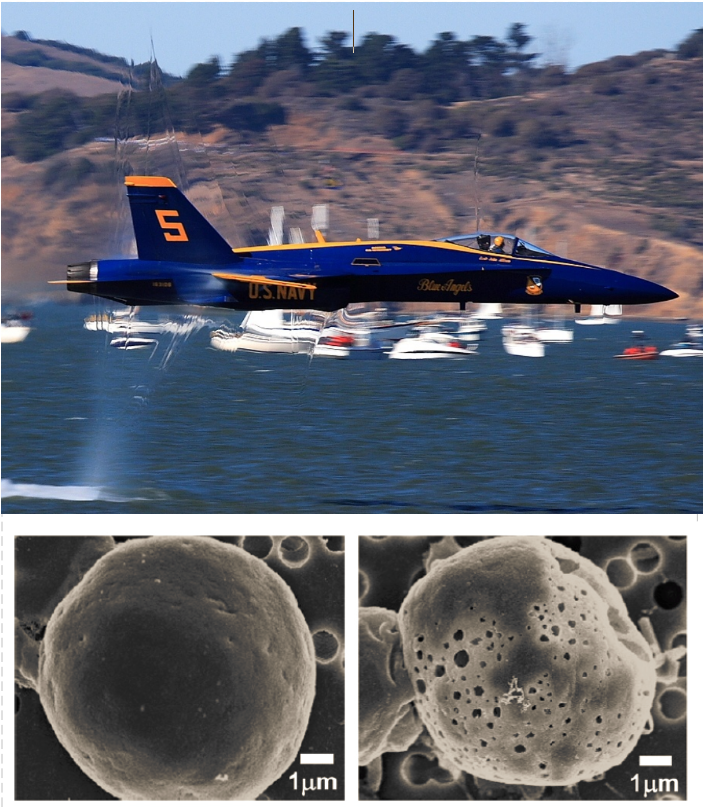
\includegraphics[width=0.825\textwidth]{Nanoshock2.png}
            \end{figure}
        \end{column}
    \end{columns}
\end{frame}


% Digital Manufacturing / 3D Printing
\begin{frame}[c]{Overview}{Digital Manufacturing - 3D Printing, Dr. S. Adami, Dr. M. Giglmaier}
    \centering
    \begin{columns}[T]
        \begin{column}{0.48\textwidth}
            % Typical SPH melt-pool simulation
            Example of a typical SPH melt-pool simulation
            \begin{itemize}
                \item Laser: P=70W, v=4m/s
                \item SPH particle: 805.000, x = 2.5$\mu$m
                \item Powder particles: 25$\mu$m, 5$\mu$m
                \item $\sim$ 1 CPUd on simple desktop workstation 
            \end{itemize}
            \begin{figure}
                \centering
                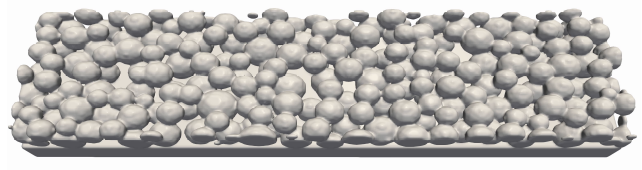
\includegraphics[width=0.85\textwidth]{3DPrinting1.png}
            \end{figure}
        \end{column}
        % Cluster and recoding of lab-size experiments
        \begin{column}{0.48\textwidth}
            % Additive cluster
            \begin{figure}
                \centering
                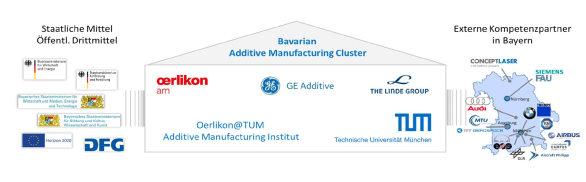
\includegraphics[width=0.65\textwidth]{3DPrintingCluster.png}
            \end{figure}
            Recording of lab-size experiment
            \begin{itemize}
                \item Inconel 718 Powder
                \item Laser: P=125W, v=2m/s
                \item Shielding gas: Argon
            \end{itemize}
            \begin{figure}
                \centering
                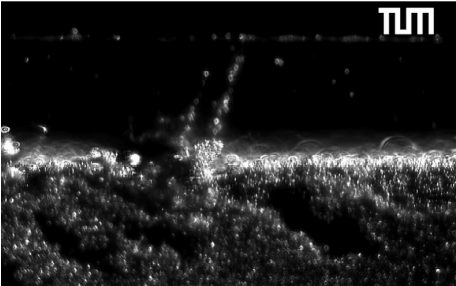
\includegraphics[width=0.55\textwidth]{3DPrinting2.png}
            \end{figure}
        \end{column}
    \end{columns}
\end{frame}



% Course outline
\section{Course Outline}

\begin{frame}[c]{Course Outline}
    \centering
    \begin{itemize}
        \item 4 Lectures
        \begin{enumerate}
            \item Foundational Knowledge
            \item Inference Engines \& Introduction to Turing.jl
            \item Hierarchical Bayesian Approaches \& Bayesian Deep Learning
            \item The Connection to Scientific Problems
        \end{enumerate}
        \item 3 Tutorials for Self-Paced Consumption
        \begin{enumerate}
            \item In-Depth Introduction to Probabilistic Programming Systems with Turing.jl
            \item Bayesian Approaches in Probabilistic Programming
            \begin{itemize}
                \item Bayesian Deep Learning
                \item Hierarchical Bayesian Modelling
            \end{itemize}
            \item Machine-Learning Based Design with Probabilistic Programming
        \end{enumerate}
    \end{itemize}
\end{frame}


% Lecture 1 breakdown
\begin{frame}[c]{Lecture 1}
    \centering
    \begin{itemize}
        \item Example Applications of Probabilistic Programming
        \begin{enumerate}
            \item \textit{ETALUMIS: Bringing Probabilistic Programming to Scientific Simulators at Scale}
            \item \textit{DreamCoder: Growing Generalizable, Interpretable Knowledge with Wake-Sleep Bayesian Program Learning}
        \end{enumerate}
        \item Why do we even need Probabilistic Programming?
        \item Underlying Theoretical Ideas
    \end{itemize}
\end{frame}


% Lecture 2 breakdown
\begin{frame}[c]{Lecture 2}
    \centering
    \begin{itemize}
        \item Approaches to Inference - the Inference Engine
        \item Probabilistic Programming Frameworks
        \item Practical Introduction to a Probabilistic Programming Framework
    \end{itemize}
\end{frame}


% Lecture 3 breakdown
\begin{frame}[c]{Lecture 3}
    \centering
    \begin{itemize}
        \item Bayesian Hierarchical Approaches
        \item Bayesian Deep Learning, including but not limited to
        \begin{itemize}
            \item Inference Networks
            \item Uncertainty Quantification
        \end{itemize}
        \item Marrying Deep Learning Frameworks with Probabilistic Programming for Type 2 Machine Learning
    \end{itemize}
\end{frame}


% Lecture 4 breakdown
\begin{frame}[c]{Lecture 4}
    \centering
    \begin{itemize}
        \item Interaction with Scientific Simulators
        \begin{itemize}
            \item What types of simulators would I want to link to?
            \item What are the hidden pitfalls?
        \end{itemize}
        \item Areas of application
        \begin{itemize}
            \item Robotics
            \item Physics
            \item Engineering
            \item Machine-Learning Based Design
        \end{itemize}
        %\item Extensive Machine-Learning Based Design Example  --> To be introduced as its own lecture at a later point
    \end{itemize}
\end{frame}



% Examples, examples, examples
\section{Example Applications of Probabilistic Programming}


% Example 1 (~16 slides?)
\subsection{ETALUMIS: Bringing Probabilistic Programming to Scientific Simulators at Scale}


% Etalumis Slide 1: Rough summary
\begin{frame}[c]{Etalumis}{Bringing Probabilistic Programming to Scientific Simulators at Scale \footnote{Baydin, A.G., Shao, L., Bhimji, W., Heinrich, L., Meadows, L., Liu, J., Munk, A., Naderiparizi, S.,
                                                                                                          Gram-Hansen, B., Louppe, G. and Ma, M., 2019, November. Etalumis: Bringing probabilistic programming
                                                                                                          to scientific simulators at scale. In Proceedings of the International Conference for High Performance
                                                                                                          Computing, Networking, Storage and Analysis (pp. 1-24).}}
    \centering
    \begin{itemize}
        \item Large scale inverse problem, where a particle simulator is inverted by probabilistically inferring
              all choices in the simulator given the desired outputs
        \begin{itemize}
            \item Developed in the context of particle simulations at CERN
        \end{itemize}
        \item First large-scale application of probabilistic programming to physical simulators in the quest
              to potentially unearth new physics \footnote{Cranmer, K., Brehmer, J. and Louppe, G., 2020. The frontier of simulation-based inference. Proceedings of the National Academy of Sciences.}
        \item Largest-scale posterior inference with 25000 latent variables at the time
        \item Amount of compute required highly dependent on the specific approach to inference and the nature of the
              simulator, i.e. latent dimensionality and intensity of the compute routine
        \begin{itemize}
            \item Only set to improve with the impeding exascale-era
        \end{itemize}
    \end{itemize}
\end{frame}


% Etalumis Slide 2: Delving into the used techniques  -> 3 page innuendo for inference compilation and a 3 page innuendo for amortized inference
\begin{frame}[c]{Etalumis}
    \centering
    \begin{itemize}
        \item Proposes a direct linking of particle physics simulators with probabilistic programming systems to trace the
              internal structure of the simulator
        \begin{itemize}
            \item Probabilistic programming system controls the random number draws of the simulator akin to samples from
                  prior distributions in Bayesian statistics
        \end{itemize}
        \item Utilizing inference compilation with three-dimensional convolutional LSTMs to guide the inference procedure
              and amortize the high computational costs of training
        \begin{itemize}
            \item Dynamic compilation, in which a core gets expanded with further neural network components as inference compilation
                  proceeds
        \end{itemize}
        \item Utilizes importance sampling in conjunction with inference compilation as approach to inference
    \end{itemize}
\end{frame}


% Etalumis Slide 3: Simulation-specific setting
\begin{frame}[c]{Etalumis}{Simulators as Probabilistic Programs}
    \centering
    \begin{itemize}
        \item A simulator execution is viewed as an execution trace, a single sample to the probabilistic programming system
        \begin{itemize}
            \item I.e. sampling is taking place in the space of execution traces
        \end{itemize}
        \item Abstracting the simulator in this way enables the following analysis
        \begin{itemize}
            \item Compute likelihoods
            \item Learn/construct surrogate models
            \item Generate training data for inference compilation
            \item Introduce other generative approaches into the loop
        \end{itemize}
        \item Enables us to guide the simulation in an intelligent fashion, using the inference network, which acts as a kind of oracle
    \end{itemize}
\end{frame}


% Etalumis Slide 4: PPX, i.e. high-level view
\begin{frame}[c]{Etalumis}
    \centering
    \begin{figure}
        \centering
        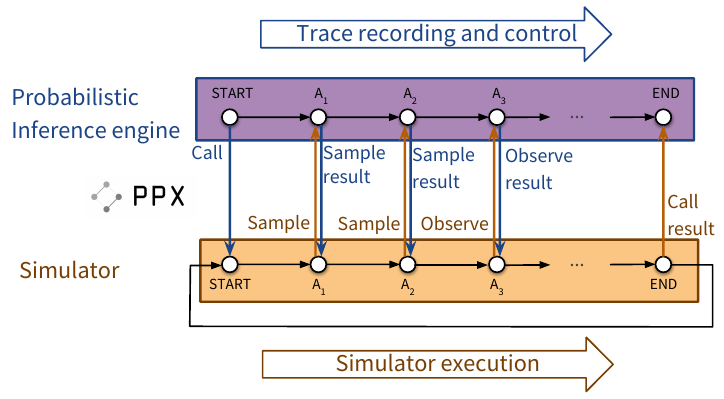
\includegraphics[width=0.8\textwidth]{PPXTrace.png}
        \caption{High-level view from the perspective of the probabilistic programming execution protocol (PPX).}
    \end{figure}
\end{frame}


% Etalumis Slide 5: Simulation and inference connection
\begin{frame}[c]{Etalumis}
    \centering
    \begin{figure}
        \centering
        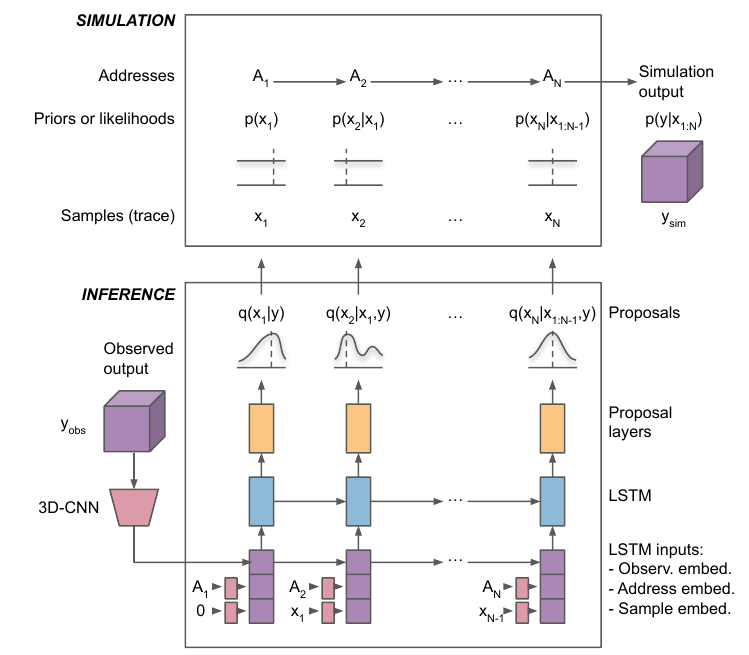
\includegraphics[width=0.549\textwidth]{ETALUMISSimulationandInference.png}
        \caption{Detailed connection between simulation and inference in the probabilistic programming-based approach.}
    \end{figure}
\end{frame}



% Amortized Inference Innuendo Slide 1
\begin{frame}[c]{Etalumis}{Recap: Amortized Inference \footnote{Gershman, S. and Goodman, N., 2014. Amortized inference in
                                                                probabilistic reasoning. In Proceedings of the annual meeting
                                                                of the cognitive science society (Vol. 36, No. 36).}
                                                      \footnote{Ritchie, D., Horsfall, P. and Goodman, N.D., 2016. Deep amortized
                                                                inference for probabilistic programs. arXiv preprint arXiv:1610.05735.}}
    \centering
    \begin{itemize}
        \item Key idea: Learn from past inferences, to make future inferences run faster
        \begin{itemize}
            \item Motivated by the brain's processing of information in context related information
        \end{itemize}
        \item Constructs a parameterized guide program, which does not necessarily need to be a neural network
        \item Traditionally probabilistic programming systems utilize a form of inference, such as Monte Carlo, dynamic programming, or
              analytic computation to approximately solve an intractable integral from scratch on every invocation
        \item Simplified by constraining the control flow of the guide to the one of the original, in opposition to previous
              program induction approaches
        \item Manual construction at the stage of the mentioned papers. $\rightarrow$ see inference compilation
    \end{itemize}
\end{frame}


% Amortized Inference Innuendo Slide 2
\begin{frame}[c]{Etalumis}{Recap: Amortized Inference}
    \centering
    % Two Column layout
    \begin{columns}[T]
        % Example dependency graph
        \begin{column}{0.4\textwidth}
            \centering
            \begin{figure}
                \centering
                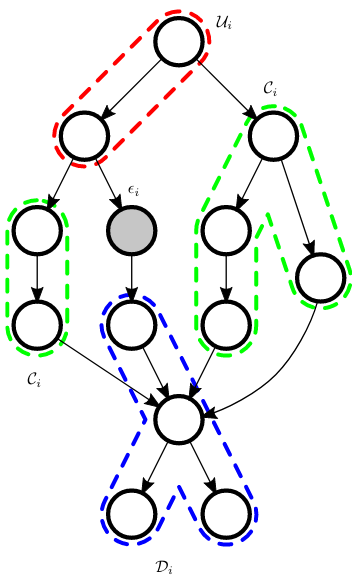
\includegraphics[width=0.7\textwidth]{AmortizedInferenceExampleGraph.png}
            \end{figure}
        \end{column}
        % Example program
        \begin{column}{0.58\textwidth}
            \centering
            \begin{figure}
                \centering
                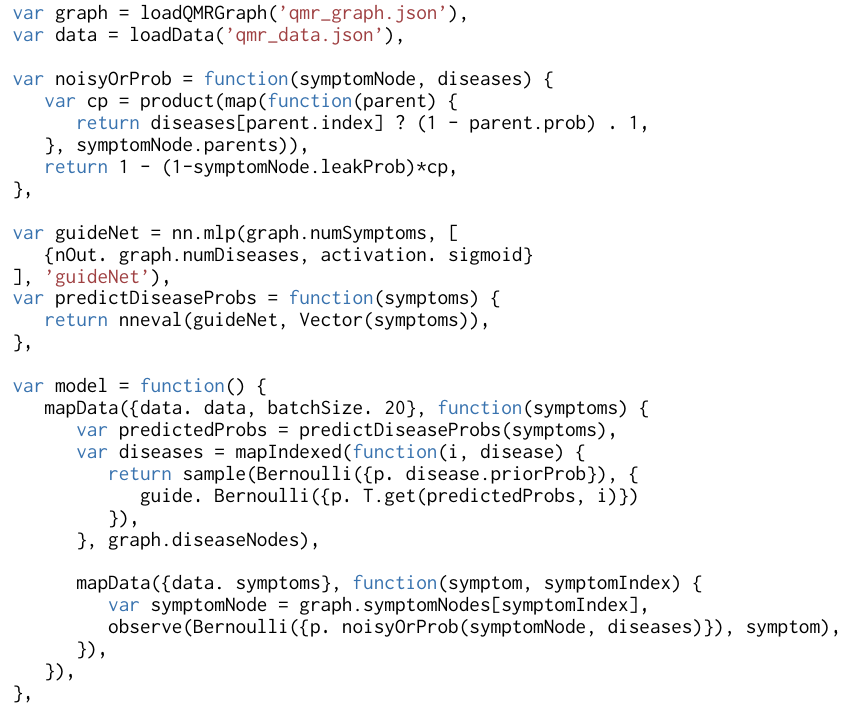
\includegraphics[width=0.85\textwidth]{AmortizedInferenceExampleProgram.png}
            \end{figure}
        \end{column}
    \end{columns}
\end{frame}


% Amortized Inference Innuendo Slide 3
\begin{frame}[c]{Etalumis}{Recap: Amortized Inference}
    \centering
    \begin{figure}
        \centering
        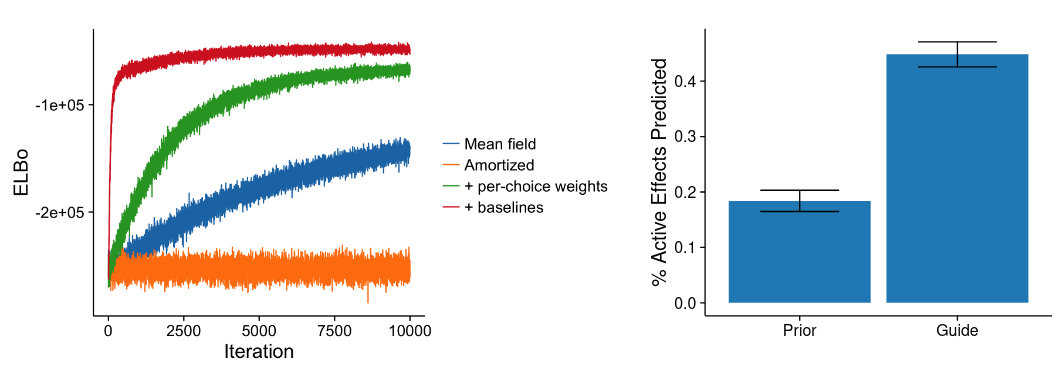
\includegraphics[width=\textwidth]{AmortizedInferenceQMR-DTPerformance.png}
        \caption{(Left) ELBo optimization progress. (Right) Percentage of test set active effects
                 correctly predicted using latent causes from either the prior or the guide program.}
    \end{figure}
\end{frame}


% Inference Compilation Innuendo Slide 1
\begin{frame}[c]{Etalumis}{Outlook: Inference Compilation \footnote{Le, T.A., Baydin, A.G. and Wood, F., 2017, April. Inference
                                                                    compilation and universal probabilistic programming. In Artificial
                                                                    Intelligence and Statistics (pp. 1338-1348).}    }
    \centering
    \begin{itemize}
        \item Uses neural networks to construct a surrogate model for the probabilistic generative model, which is subsequently
              used at inference time as a custom proposal distribution to avoid sampling from the actual generative model
        \item Intuition is that the cost of constructing the surrogate can be amortized at inference time and be lower
              inference from the underlying generative model
        \begin{itemize}
            \item Need to watch out for sample diversity and out-of-distribution samples 
        \end{itemize}
        \item Proposes adaptive neural network architecture with a recurrent core and embedding and proposal layers specified
              by the probabilistic program
        \item Approach is model-agnostic
    \end{itemize}
\end{frame}


% Inference Compilation Innuendo Slide 2
\begin{frame}[c]{Etalumis}{Outlook: Inference Compilation}
    \centering
    \begin{figure}
        \centering
        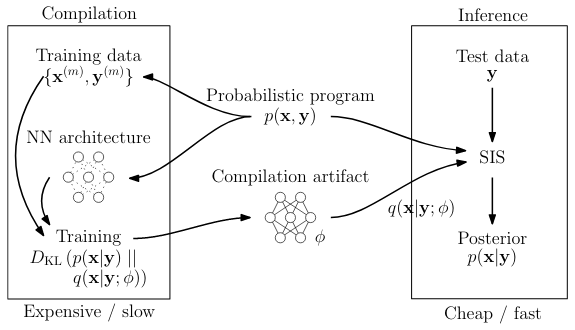
\includegraphics[width=0.7\textwidth]{InferenceCompilationSketch.png}
        \caption{Automatic construction of a neural network surrogate, which is then trained with data generated by the probabilistic
                 program to eventually act as the proposal distribution at inference time.}
    \end{figure}
\end{frame}


% Inference Compilation Innuendo Slide 3
\begin{frame}[c]{Etalumis}{Outlook: Inference Compilation}
    \centering
    \begin{figure}
        \centering
        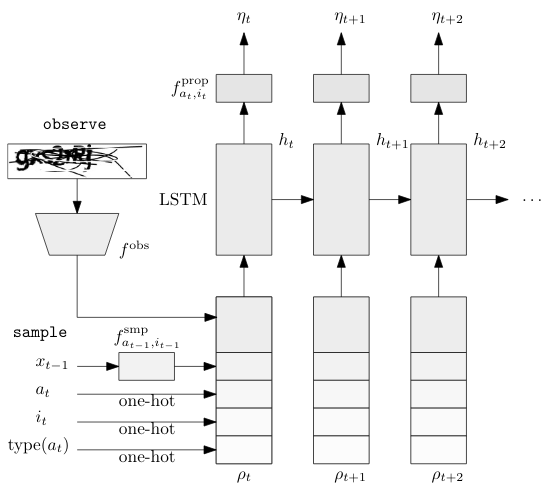
\includegraphics[width=0.4\textwidth]{InferenceCompilationPractice.png}
        \caption{Example application for captcha solving based on probabilistic generative models for the captchas.
                 With the LSTM at its core, required embeddings for the respective are attached adaptively.}
    \end{figure}
\end{frame}


% Etalumis Slide 6: Distributed training algorithm
\begin{frame}[c]{Etalumis}
    \centering
    \begin{figure}
        \centering
        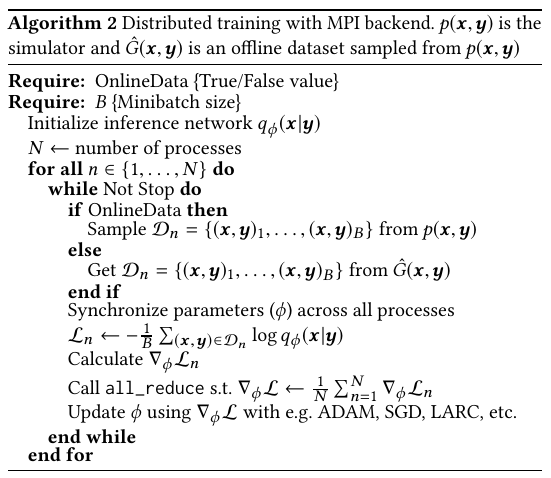
\includegraphics[width=0.6\textwidth]{EtalumisTrainingAlgorithm.png}
    \end{figure}
\end{frame}


% Etalumis Slide 7: Posteriors of the targeted particle distributions
\begin{frame}[c]{Etalumis}
    \centering
    \begin{figure}
        \centering
        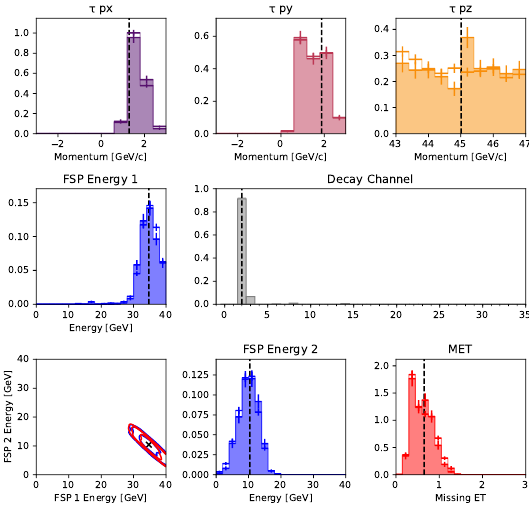
\includegraphics[width=0.5\textwidth]{EtalumisParticlePosteriors.png}
        \caption{Posteriors obtained with random-walk Metropolis Hasting (filled histograms) and inference compilation (outline histograms) and
                 ground truth values (dashed vertical lines).}
    \end{figure}
\end{frame}


% Etalumis Slide 8: Scaling on Edison and Cori
\begin{frame}[c]{Etalumis}
    \centering
    % Two columns for two scaling plots
    \begin{columns}[T]
        % Scaling on Cori
        \begin{column}{0.48\textwidth}
            \centering
            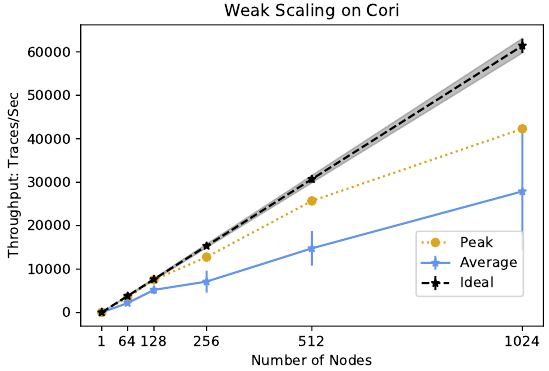
\includegraphics[width=0.9\textwidth]{EtalumisScalingCori.png}
        \end{column}
        % Scaling on Edison
        \begin{column}{0.48\textwidth}
            \centering
            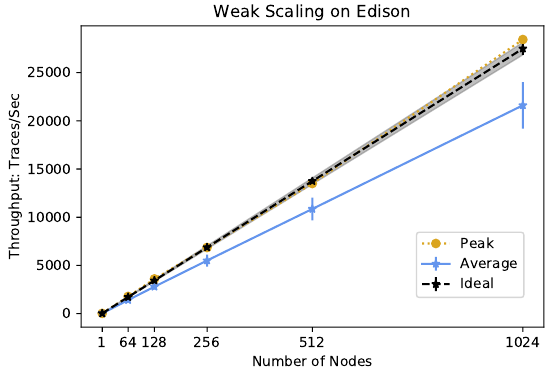
\includegraphics[width=0.9\textwidth]{EtalumisScalingEdison.png}
        \end{column}
    \end{columns}
    \vspace{1cm}
    \begin{itemize}
        \item Moving to supercomputer scale for massive-scale inference to be able to generate the necessary
              number of simulations for the inference compilation to be successful.
    \end{itemize}
\end{frame}


% Etalumis Slide 9: Summary
\begin{frame}[c]{Etalumis}
    \centering
    \begin{itemize}
        \item First probabilistic programming system to link to scientific simulators at scale to enable large-scale
              posterior inference on a supercomputing-scale
        \begin{itemize}
            \item Can only ever capture the processes encapsulated in the simulator
        \end{itemize}
        \item Introduces a probabilistic programming execution protocol to link to scientific simulators
        \item To make inference tractable it needs to rely on techniques, such as amortization through inference
              compilation, which essentially constructs an oracle
        \item Pushes the frameworks to the extreme with communication requirements and data exchange between computing instances
    \end{itemize}
\end{frame}



% Example 2 (~10 slides?)
\subsection{DreamCoder: Growing Generalizable, Interpretable Knowledge with Wake-Sleep Bayesian Program Learning}

% DreamCoder Slide 1: Rough summary
\begin{frame}[c]{DreamCoder \footnote{Ellis, K., Wong, C., Nye, M., Sable-Meyer, M., Cary, L., Morales, L., Hewitt, L., Solar-Lezama, A. and Tenenbaum, J.B., 2020. DreamCoder: Growing generalizable, interpretable knowledge with wake-sleep Bayesian program learning. arXiv preprint arXiv:2006.08381.}}{Growing Generalizable, Interpretable Knowledge with Wake-Sleep Bayesian Program Learning}
    \centering
    \begin{itemize}
        \item Constructs domain-specific languages (DSLs) for scientific problems combined with a neural network,
              which embodies a learned domain-specific search strategy
        \begin{itemize}
            \item Learns both the system prior and the needed inference algorithm
        \end{itemize}
        \item Practically constructs a library of symbolic abstractions in a wake-sleep manner and applies said library
              to the solving of the chosen problem at hand
        \item Wake-sleep learning % reference needed here
        \begin{itemize}
            \item During \textit{sleep} the system consolidates its abstractions from the programs found during \textit{wake}
                  and improves upon the neural network recognition model by imagining new samples
            \item During \textit{wake} the generative model is exploited on the problem domain to find the programs with the
                  highest posterior probability
        \end{itemize}
    \end{itemize}
\end{frame}


% Slide 2: Knowledge-Hierarchy and Probabilistic Inference
\begin{frame}[c]{DreamCoder}
    \centering
    \begin{itemize}
        \item Knowledge is accumulated in a multilayered hierarchy with knowledge and skills being
              successively learned over time, i.e. the knowledge is bootstrapped from very simple
              examples to ever more complex cases
        \item Can be broken down to a probabilistic inference procedure, i.e. observing task $X$ and
              inferring program $\rho_{x}$ to solve task $x \in X$ combined with a prior distribution
              over program, which migh solve tasks in the domain
        \begin{align*}
            \rho_{x} &= \underset{\substack{\rho: \\ Q(\rho|x) \text{ is large}}}{\arg \max} P[\rho | x, L] \propto P[x | \rho ] P[\rho | L], \text{ for each task } x \in X &Wake \\
            L &= \underset{L}{\arg \max} P[L] \prod_{x \in X} \underset{\rho \text{ a refactoring of } \rho_{x}}{\max} P[x | \rho] P[\rho | L] &Sleep: Abstraction \\
            \text{Train } &Q(\rho | x) \approx P[\rho | x, L], \text{ where } x \sim X \text{ ('replay') or } x \sim L \text{ ('fantasy')} & Sleep: Dreaming
        \end{align*}
    \end{itemize}
\end{frame}


% DreamCoder Slide 3: Overall algorithm
\begin{frame}[c]{DreamCoder}
    \centering
    \begin{figure}
        \centering
        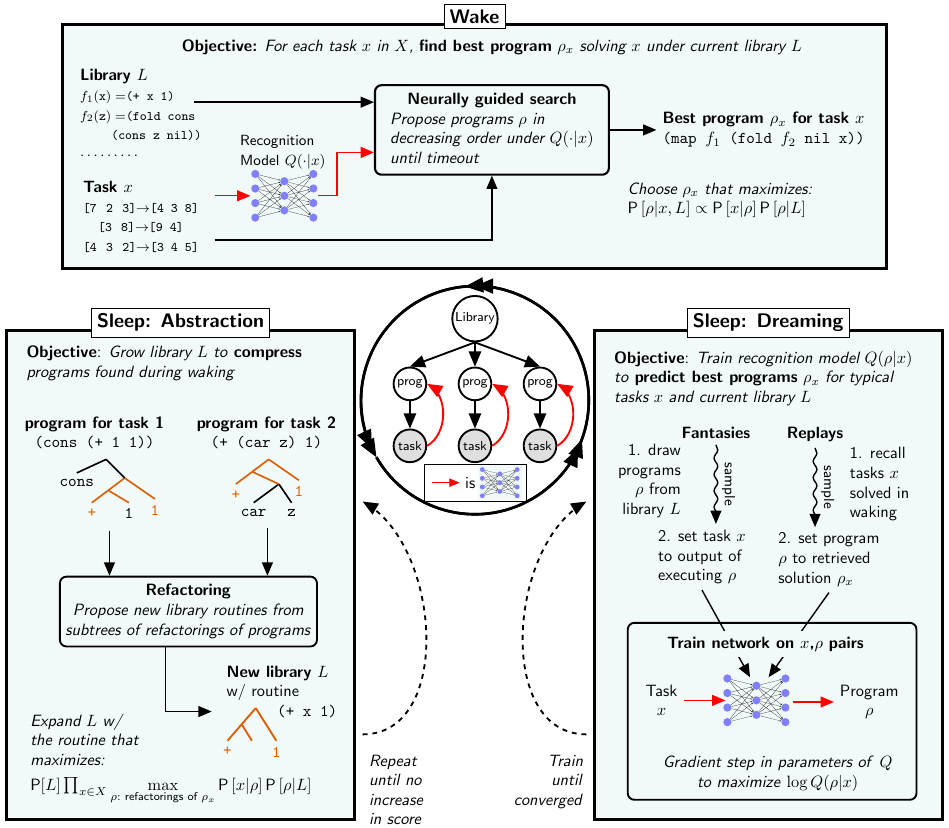
\includegraphics[width=0.5\textwidth]{DreamCoderAlgorithmCycle.png}
        \caption{Algorithm Cycle of DreamCoder}
    \end{figure}
\end{frame}


% DreamCoder Slide 4: Algorithm
\begin{frame}[c]{DreamCoder}
    \centering
    \begin{figure}
        \centering
        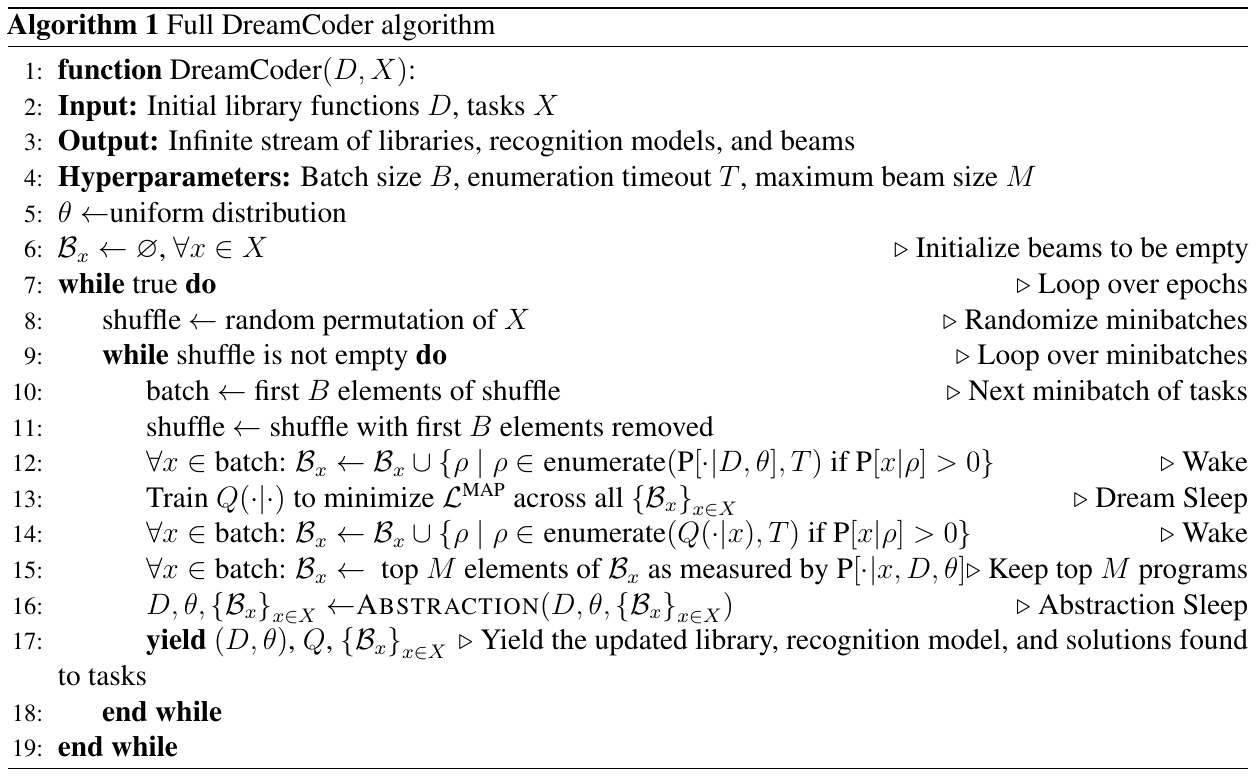
\includegraphics[width=0.7\textwidth]{DreamCoderAlgo.png}
    \end{figure}
\end{frame}


% DreamCoder Slide 5: Algorithm Structure
\begin{frame}[c]{DreamCoder}
    \centering
    \begin{figure}
        \centering
        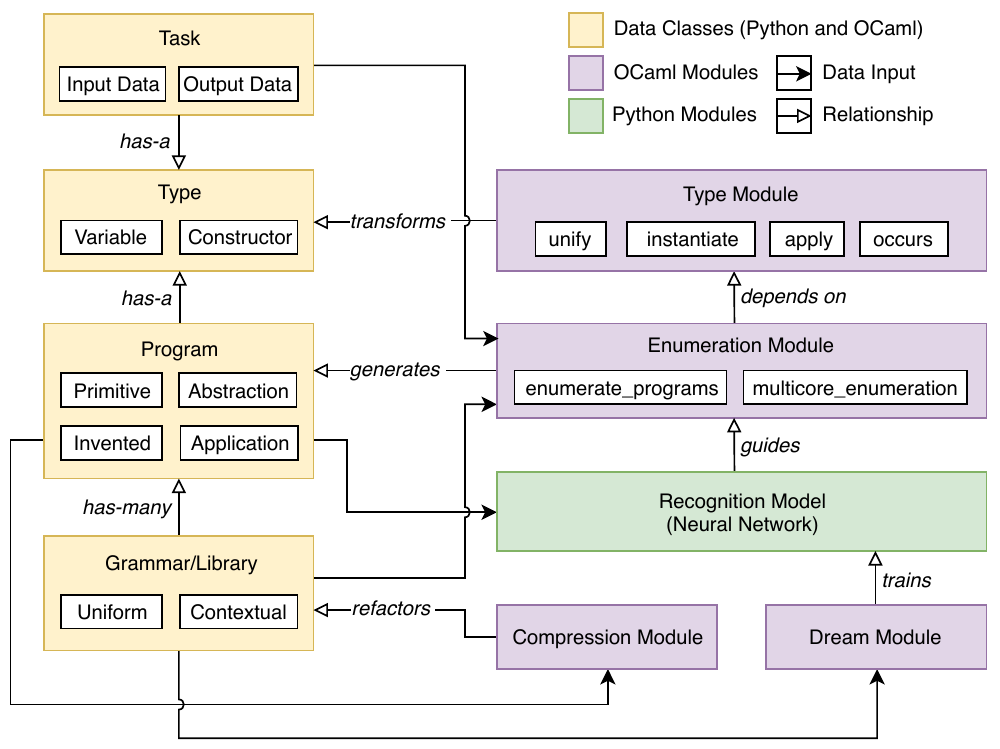
\includegraphics[width=0.6\textwidth]{DreamCoderDataClasses.png}
        \caption{Different data-classes in DreamCoder.}
    \end{figure}
\end{frame}


% DreamCoder Slide 6: Program Flowchart
\begin{frame}[c]{DreamCoder}
    \centering
    \begin{figure}
        \centering
        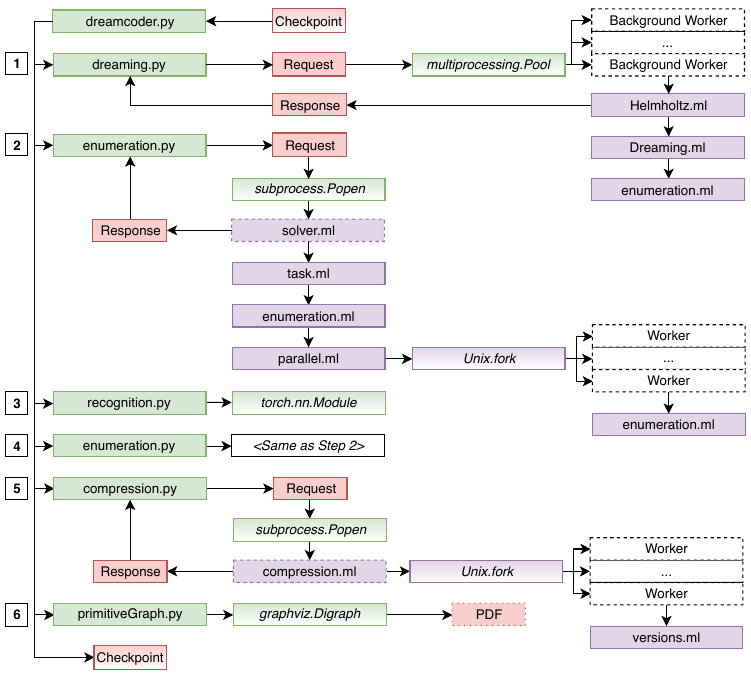
\includegraphics[width=0.5\textwidth]{DreamCoderProgramFlowchart.png}
        \caption{Program Flowchart: Phase 1, Dreaming. Phase 2, 1st Program Enumeration. Phase 3, Recognition Model Training.
                 Phase 4, 2nd Program Enumeration. Phase 5, Abstraction (Compression). Phase 6, Library Visualization.}
    \end{figure}
\end{frame}


% DreamCoder Slide 7: Helmholtz Machine Innuendo 1
\begin{frame}[c]{Recap: Helmholtz Machine \footnote{Graves, A., Wayne, G. and Danihelka, I., 2014. Neural turing machines. arXiv preprint arXiv:1410.5401.}
                                          \footnote{YouTube: DeepMind x UCL | Deep Learning Lectures | 8/12 | Attention and Memory in Deep Learning}}
    \centering
    % Two columns, text on the left, images on the right
    \begin{columns}[T]
        % Column for text explanation
        \begin{column}{0.48\textwidth}
            \begin{itemize}
                \item Couples neural networks with external memory, which is accessed through an
                      internal attention mechanism
                \begin{itemize}
                    \item Iteratively modify the state of the network through its memory mechanism
                \end{itemize}
                \item Can infer simple algorithms from data
                \item Structure
                \begin{itemize}
                    \item Controller is a neural network
                    \item Heads select the part of the memory to access
                    \item Memory is essentially a large matrix
                \end{itemize}
            \end{itemize}
        \end{column}
        % Column for contextual images
        \begin{column}{0.48\textwidth}
            \begin{figure}
                \centering
                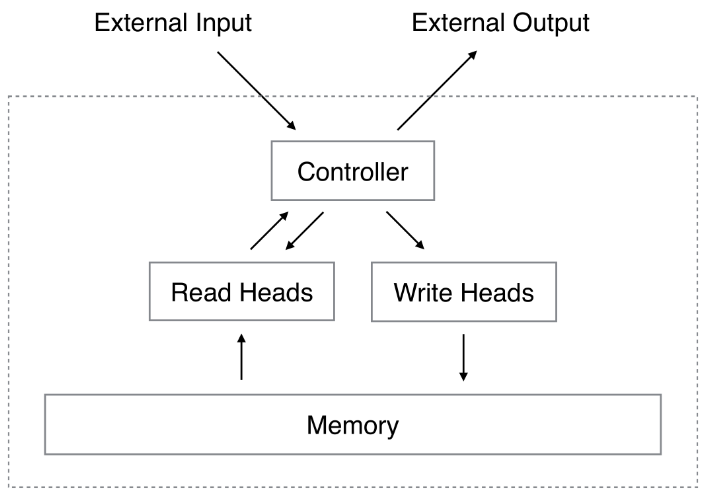
\includegraphics[width=0.9\textwidth]{NeuralTuringMachineArchitecture.png}
            \end{figure}
        \end{column}
    \end{columns}
\end{frame}


% DreamCoder Slide 8: Helmholtz Machine Innuendo 2
\begin{frame}[c]{Recap: Helmholtz Machine}
    \centering
    \begin{itemize}
        \item Heavily relies on selection attention, whee the controller emits a distribution over the memory matrix,
              which then defines content- and location-based attention mechanisms \footnote{Lilian Weng's review of attention: https://lilianweng.github.io/lil-log/2018/06/24/attention-attention.html}
        \item Content-based:
        \begin{itemize}
            \item A key vector is compared to each memory location
        \end{itemize}
        \item Location-based:
        \begin{itemize}
            \item Use a shift kernel in conjunction with the weighting to shift to a new location in memory
        \end{itemize}
        \item Results in three different interaction modes:
        \begin{enumerate}
            \item Content key only
            \item Content and location
            \item Location only
        \end{enumerate}
    \end{itemize}
\end{frame}


% DreamCoder Slide 9: Helmholtz Machine Innuendo 3  <- Priority sort
\begin{frame}[c]{Recap: Helmholtz Machine}{Example: Priority Sort}
    \centering
    % Two columns
    \begin{columns}[T]
        % Text describing the case
        \begin{column}{0.48\textwidth}
            \vspace{0.55cm}
            \begin{itemize}
                \item Learns algorithm to sort data from a sequence of random binary vectors and their
                      respective scalar priority rating
            \end{itemize}
        \end{column}
        % Illustration of the case
        \begin{column}{0.48\textwidth}
            \begin{figure}
                \centering
                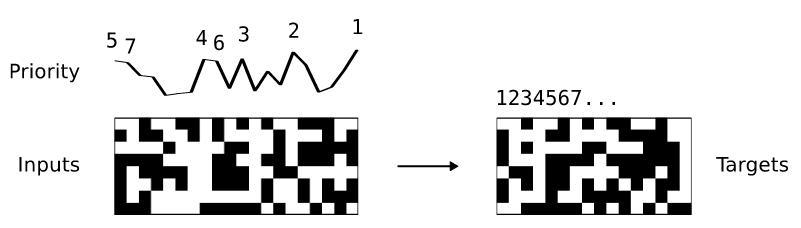
\includegraphics[width=\textwidth]{NTMPrioritySortIllustration.png}
            \end{figure}
        \end{column}
    \end{columns}
    % Memory of the neural turing machine during the priority sort task
    \begin{figure}
        \centering
        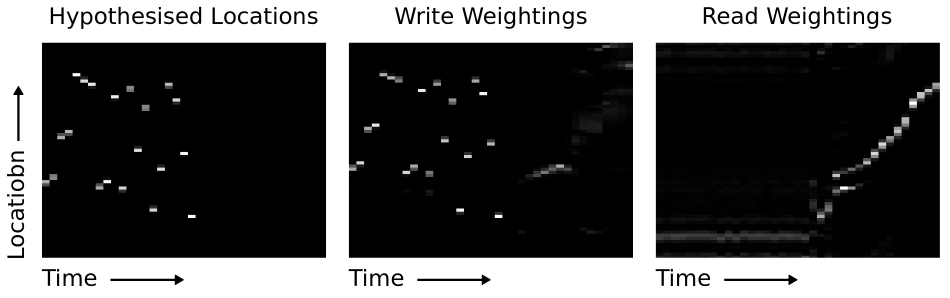
\includegraphics[width=0.85\textwidth]{NTMPrioritySortMemoryAccess.png}
    \end{figure}
\end{frame}


% DreamCoder Slide 10: Differentiable Neural Computers (Outlook)
\begin{frame}[c]{Outlook: Differentiable Neural Computer \footnote{Graves, A., Wayne, G., Reynolds, M., Harley, T., Danihelka, I., Grabska-Barwińska, A., Colmenarejo,
                                                                   S.G., Grefenstette, E., Ramalho, T., Agapiou, J. and Badia, A.P., 2016. Hybrid computing using a
                                                                   neural network with dynamic external memory. Nature, 538(7626), pp.471-476.}}
    \centering
    \begin{itemize}
        \item Successor architecture to the neural turing machine with new attention mechanisms
        \item Specifically geared towards applications in graphs $\longrightarrow$  more on this later!
    \end{itemize}
    \begin{figure}
        \centering
        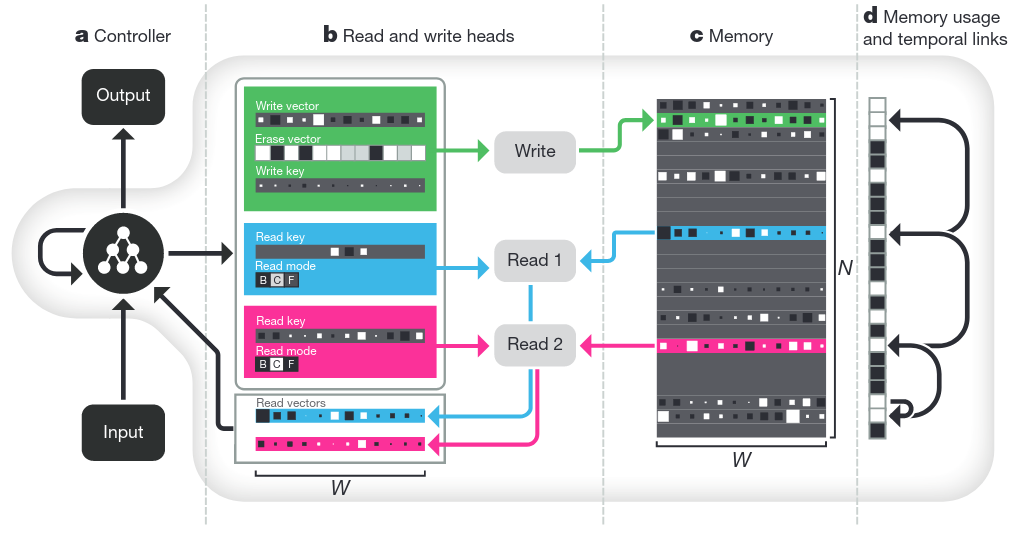
\includegraphics[width=0.55\textwidth]{DifferentiableNeuralComputerArchitecture.png}
    \end{figure}
\end{frame}


% DreamCoder Slide 10: Compositional Nature
\begin{frame}[c]{DreamCoder}
    \centering
    \begin{itemize}
        \item Due to its compositional nature, representations of problems can be bootstrapped from earlier, simpler version of
              the scientific task to more and more complex settings
    \end{itemize}
    \vspace{1cm}
    \begin{figure}
        \centering
        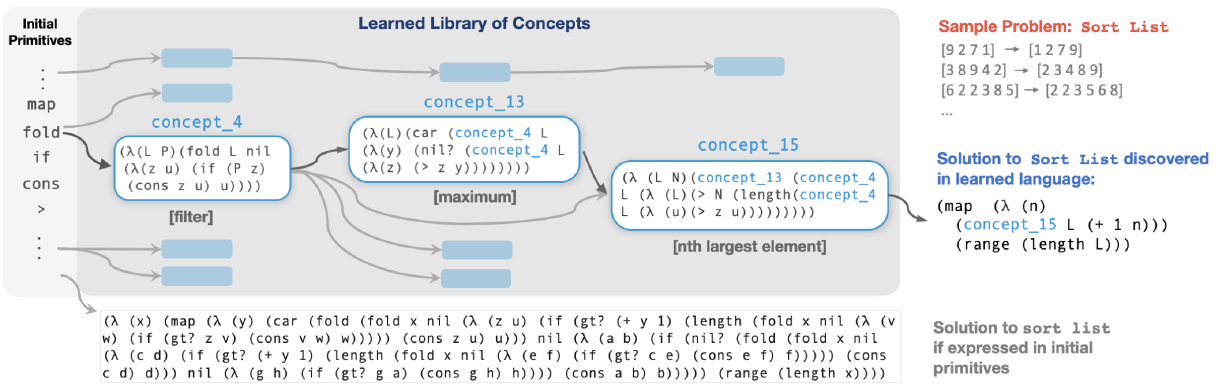
\includegraphics[width=\textwidth]{DreamCoderCompositionality.png}
    \end{figure}
\end{frame} 


% DreamCoder Slide 11: Applications of the Algorithm
\begin{frame}[c]{DreamCoder}{Applications}
    % Three columns of potential applications
    \begin{columns}[T]
        % First columns
        \begin{column}{0.33\textwidth}
            % List Processing
            \begin{figure}
                \centering
                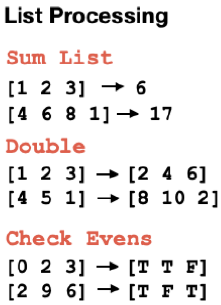
\includegraphics[height=0.35\textheight]{DreamCoderApp1.png}
            \end{figure}
            % Logo Graphics
            \begin{figure}
                \centering
                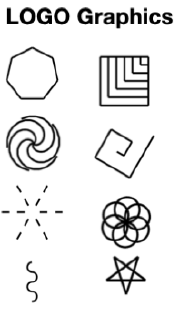
\includegraphics[height=0.35\textheight]{DreamCoderApp4.png}
            \end{figure}
        \end{column}
        % Second column
        \begin{column}{0.33\textwidth}
            % Block Towers
            \begin{figure}
                \centering
                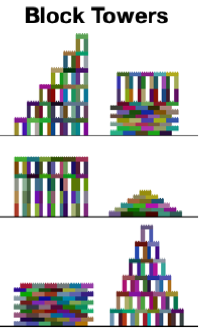
\includegraphics[height=0.35\textheight]{DreamCoderApp5.png}
            \end{figure}
            % Symbolic Regression
            \begin{figure}
                \centering
                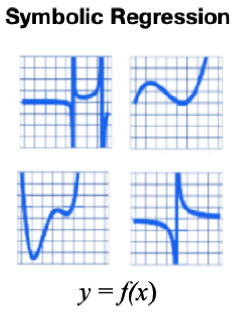
\includegraphics[height=0.35\textheight]{DreamCoderApp6.png}
            \end{figure}
        \end{column}
        % Third column
        \begin{column}{0.33\textwidth}
            % Recursive Programming
            \begin{figure}
                \centering
                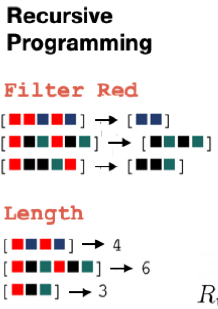
\includegraphics[height=0.35\textheight]{DreamCoderApp7.png}
            \end{figure}
            % Physical Laws
            \begin{figure}
                \centering
                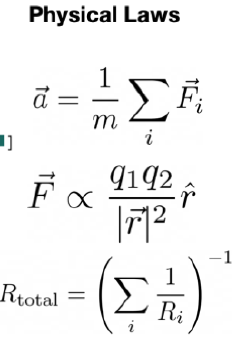
\includegraphics[height=0.35\textheight]{DreamCoderApp8.png}
            \end{figure}
        \end{column}
    \end{columns}
\end{frame}


% DreamCoder Slide 12: Applications of the Algorithm
\begin{frame}[c]{DreamCoder}{Applications}
    \centering
    \begin{figure}
        \centering
        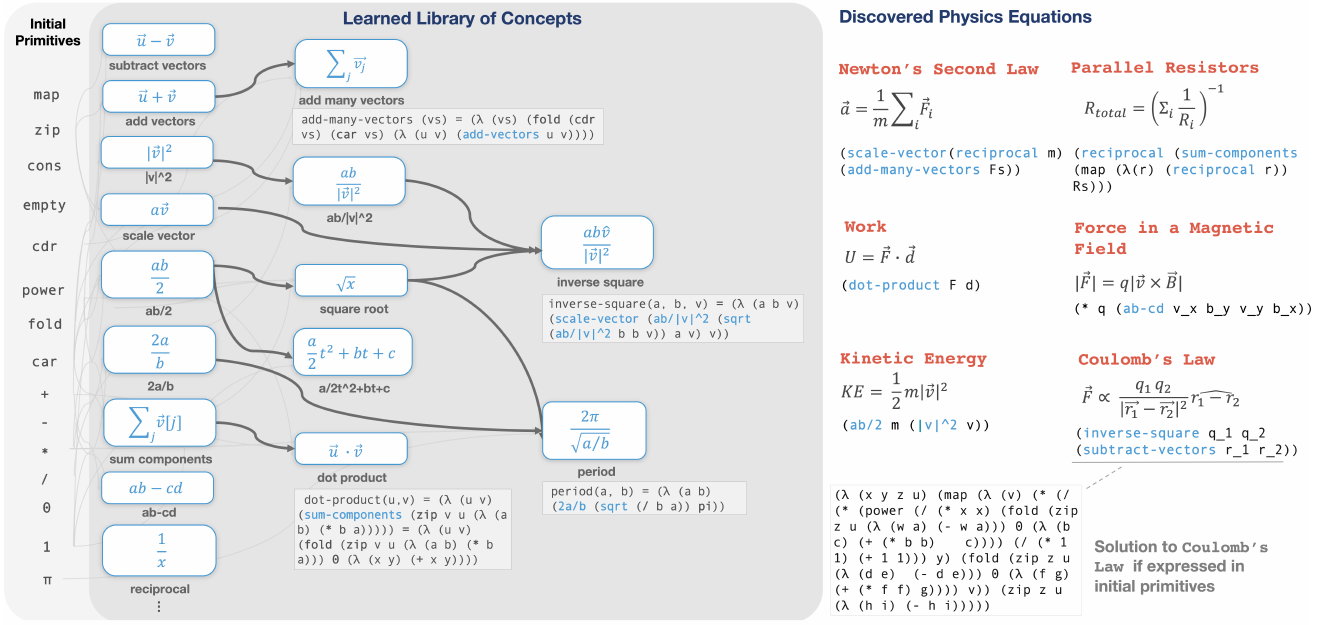
\includegraphics[width=0.95\textwidth]{DreamCoderApplication1.png}
        \caption{Learned library for physics equations.}
    \end{figure}
\end{frame}


% DreamCoder Slide 13: Applications of the Algorithm
\begin{frame}[c]{DreamCoder}{Applications}
    \centering
    \begin{figure}
        \centering
        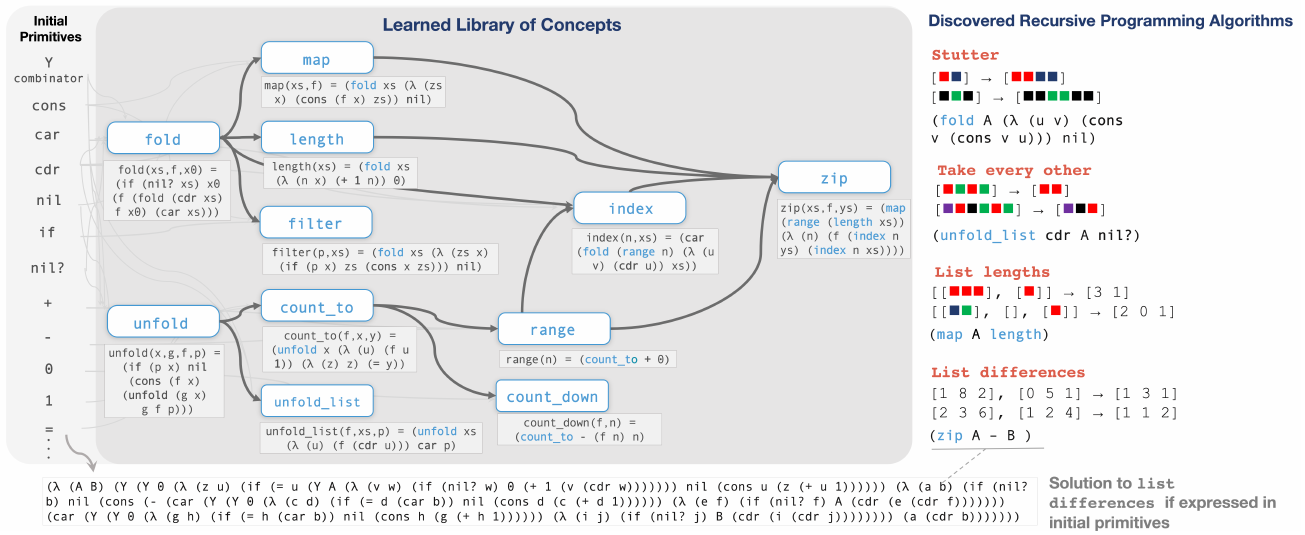
\includegraphics[width=0.95\textwidth]{DreamCoderApplication2.png}
        \caption{Learned library for recursive programming algorithm.}
    \end{figure}
\end{frame}


% DreamCoder Slide 14: Applications of the Algorithm
\begin{frame}[c]{DreamCoder}{Applications}
    \centering
    \begin{figure}
        \centering
        \includegraphics[width=\textwidth]{DreamCoderApplication3.png}
        \caption{Learned library for LOGO graphics.}
    \end{figure}
\end{frame}


% DreamCoder Slide 15: Applications of the Algorithm
\begin{frame}[c]{DreamCoder}{Applications}
    \centering
    \begin{figure}
        \centering
        \includegraphics[width=0.65\textwidth]{DreamCoderApplication4.png}
        \caption{Learned library for list processing.}
    \end{figure}
\end{frame}


% DreamCoer Slide 16: Summary
\begin{frame}[c]{DreamCoder}{Take-Aways}
    \centering
    \begin{itemize}
        \item Combining probabilistic programming with a DSL-learning procedure and novel probabilistic inference procedure
              to iteratively learn to represent a problem's domain allows one to gain the ability to solve a problem
        \item Such applications require highly complex codebase structures across multiple languages
        \item For more complex examples reliant on a highly efficient inference procedure
    \end{itemize}
\end{frame}




% Why Do We even Need Probabilistic Programming? (5-10 slides)
\section{Why Do We even Need Probabilistic Programming?}


% The Why: Slide 1
\begin{frame}[c]{Why Do We Need Probabilistic Programming?}
    \centering
    \LARGE{The Myth of Probabilistic Programming \\ \textbf{Automated Inference} \\ Not solved for high-dimensions and modern probabilistic models}
\end{frame}


% The Why: Slide 2
\begin{frame}[c]{Why Do We Need Probabilistic Programming?}
    \centering
    \LARGE{Move away from handcoded inference routines to fast, verified ones for \textbf{reproducibility} and \textbf{focus on science}}
\end{frame}


% The Why: Slide 3
\begin{frame}[c]{Why Do We Need Probabilistic Programming?}
    \centering
    \LARGE{\textbf{Accelerate} the probabilistic modelling research cycle}
\end{frame}


% The Why: Slide 4
\begin{frame}[c]{Why Do We Need Probabilistic Programming?}
    \centering
    \LARGE{Natively express \textbf{uncertainties} over our model and workflow.}
\end{frame}


% The Why: Slide 5
\begin{frame}[c]{Why Do We Need Probabilistic Programming?}
    \centering
    \LARGE{Express ever more \textbf{complex probabilistic models}}
\end{frame}


% The Why: Slide 6
\begin{frame}[c]{Why Do We Need Probabilistic Programming?}
    \centering
    \LARGE{Express probabilistic models \textbf{as succinctly as possible}}
\end{frame}


% The Why: Slide 7
\begin{frame}[c]{Why Do We Need Probabilistic Programming?}
    \centering
    \LARGE{\textbf{Lower the barrier of entry} to Bayesian analysis for data-scientists, engineers, etc.}
\end{frame}



% Underlying Theoretical Ideas (40 slides?)
\section{Underlying Theoretical Ideas}








%
%\AERbeamerSetFooterText{References}%
%\begin{frame}[allowframebreaks]{References}%
%    \printbibliography[heading=none]%
%\end{frame}%
%
% End with titlepage
%\AERbeamerTitlePageDefault%
%
%
\end{document}%
%
%
